\documentclass[xcolor=dvipsnames]{beamer}
%\usepackage[czech]{babel}
\usepackage[utf8]{inputenc}
%balíček na A4
\usepackage{amsthm}
\usepackage{amsmath}
\usepackage{amsbsy}
\usepackage{amssymb}

\usepackage{graphicx}

%\usepackage{mathpazo}

%\usepackage[mathlf]{MinionPro}
\usepackage{sansmathfonts}
%\usepackage[mathlf,textlf]{MyriadPro}
%\usepackage{mathpazo}
\usepackage[small]{eulervm}
%\usepackage{newtxmath}

\usepackage{mathtools}
\usepackage{booktabs}
\usepackage{caption}
\usepackage{subcaption}
\usepackage{setspace}
\usepackage{array}
\usepackage{tabularx}
\usepackage{pbox}
\usepackage{mathpartir} %proof trees
\usepackage{listings}
\usepackage{xcolor}

\usepackage{tikz}
\tikzset{
   invisible/.style={opacity=0},
   visible on/.style={alt=#1{}{invisible}},
   blank/.style={},
   red on/.style={alt={#1{fill=red!10}{blank}}},
   alt/.code args={<#1>#2#3}{%
     \alt<#1>{\pgfkeysalso{#2}}{\pgfkeysalso{#3}} % \pgfkeysalso doesn't change the path
   },
 }

\captionsetup{compatibility=false}
%\renewcommand{\arraystretch}{1}
%\hypersetup{pdfpagemode={FullScreen}}

\makeatletter
    \newenvironment{withoutheadline}{
        \setbeamertemplate{headline}[default]
        \def\beamer@entrycode{\vspace*{-\headheight}}
    }{}
\makeatother

\title{Unsatisfiability Proofs}
\author{Henrich Lauko \vspace{-0.3cm}}
\institute{IA072 -- Seminar on Concurrency \vspace{1cm}}
\date{\today}

\usetheme{Antibes}
\setbeamertemplate{headline}{}
\setbeamertemplate{navigation symbols}{}%remove navigation symbols

\setbeamertemplate{footline}[frame number]

\definecolor{foreground}{RGB}{255,255,255}
\definecolor{background}{RGB}{24,24,24}
% \definecolor{title}{RGB}{107,174,214}
\definecolor{title}{RGB}{255,255,255}
\definecolor{main}{RGB}{39,66,96}
\definecolor{gray}{RGB}{155,155,155}
\definecolor{subtitle}{RGB}{102,255,204}
\definecolor{hilight}{RGB}{233,140,5}
\definecolor{vhilight}{RGB}{251,95,37}

\setbeamercolor{titlelike}{fg=title,bg=main}
\setbeamercolor{subtitle}{fg=subtitle}
\setbeamercolor{institute}{fg=gray}
%\setbeamercolor{normal text}{fg=foreground,bg=background}

\setbeamercolor*{block title}{fg=white, bg=main}
\setbeamercolor*{block body}{fg=black, bg=main!5}
\setbeamercolor*{block title example}{fg=white, bg=vhilight!65}
\setbeamercolor*{block body example}{fg=black, bg=vhilight!10}

\setbeamercolor{item}{fg=main} % color of bullets
%\setbeamercolor{subitem}{fg=gray}
\setbeamercolor{alerted text}{fg=hilight}
\setbeamercolor{description item}{fg=hilight}
%\setbeamercolor{itemize/enumerate subbody}{fg=gray}
\setbeamertemplate{itemize subitem}{{\textendash}}
\setbeamerfont{itemize/enumerate subbody}{size=\small}
\setbeamerfont{itemize/enumerate subitem}{size=\small}

\DeclareSymbolFont{operators}{\encodingdefault}{ppl}{m}{n}
\DeclareMathAlphabet{\mathbf}{\encodingdefault}{ppl}{bx}{n}
\DeclareMathAlphabet{\mathit}{\encodingdefault}{ppl}{m}{it}

\let\otp\titlepage
\renewcommand{\titlepage}{\otp\addtocounter{framenumber}{-1}}

\lstset{ %this is the stype
        mathescape=true,
        frame=tB,
        numbers=left,
        numberstyle=\tiny,
        basicstyle={\ttfamily\scriptsize},
        keywordstyle=\color{vhilight}\bfseries,
        keywords={for, do, forall, then, let,  input, output, return, datatype, function, in, if, else, foreach, while, begin, end, SAT, UNSAT, CONFLICT, } %add the keywords you want, or load a language as Rubens explains in his comment above.
        numbers=left,
        xleftmargin=.04\textwidth,
		escapeinside={<@}{@>}
    }

\newcommand{\sat}{\textcolor{Green}}
\newcommand{\unsat}{\textcolor{Red}}

\newcommand\Wider[2][3em]{%
\makebox[\linewidth][c]{%
  \begin{minipage}{\dimexpr\textwidth+#1\relax}
  \raggedright#2
  \end{minipage}%
  }%
}

\begin{document}

\begin{frame}[plain]
 \titlepage
\end{frame}

\section{Unsatisfiability proofs}
\begin{frame}
  \frametitle{Is SAT solver credible?}
    Possible results:
    \begin{itemize}
        \item SAT
        \item UNSAT
        \item TIMEOUT
    \end{itemize}
\end{frame}

\begin{frame}
  \frametitle{Criteria on unsatisfiability proofs}
    \begin{itemize}[<+->]
        \item easily checkable
        \item small/reasonable size
        \item proof checking quicker than solver
        \item proof production not slowing down the solver
        \item minimize modifications of solver
    \end{itemize}
\end{frame}

\begin{frame}
  \frametitle{Resolution}
  \textbf{Resolution rule:}
  \begin{mathpar} \inferrule*[Right=$x$]{x \vee C \\ \neg x \vee D}{C \vee D} \end{mathpar}

  We write $(x \vee C) \diamond ( \neg x \vee D) = (C \vee D)$.

  \pause
  \bigskip
  \textbf{Resolution chain}
  \[
      ((a \vee c) \diamond (\neg a \vee b)) \diamond (\neg a \vee \neg b) = (\neg a \vee c)
  \]

  Resolution chains are computed from left.
\end{frame}

\begin{frame}[t]
  \frametitle{Resolution proofs -- TraceCheck proof format}
	\[
        \varphi = (\neg b \vee c) ~\wedge~ (a \vee c) ~\wedge~
                  (\neg a \vee b) ~\wedge~ (\neg a \vee \neg b) ~\wedge~
                  (a \vee \neg b) ~\wedge~ (b \vee \neg c)
    \]

    \pause
    \begin{columns}
	\begin{column}{0.5\textwidth}
        \[
          (\neg a \vee \neg b) \diamond (a \vee \neg b) = \neg b
        \]

        \[
          (a \vee c) \diamond (\neg a \vee  b) \diamond (\neg b \vee c) = c
        \]

        \[
          (b \vee \neg c) \diamond (\neg b) \diamond (c) = \emptyset
        \]
	\end{column}
	\pause
    \begin{column}{0.5\textwidth}
		\begin{table}
		\begin{tabular}{rrrllll}
		\textbf{1} & -2 & 3          & 0          & \textbf{0} &            &            \\
		\textbf{2} & 1  & 3          & 0          & \textbf{0} &            &            \\
		\textbf{3} & -1 & 2          & 0          & \textbf{0} &            &            \\
		\textbf{4} & -1 & -2         & 0          & \textbf{0} &            &            \\
		\textbf{5} & 1  & -2         & 0          & \textbf{0} &            &            \\
		\textbf{6} & 2  & -3         & 0          & \textbf{0} &            &            \\
		           &    &            &            &            &            &            \\
        \textbf{7} & -2 & 0          & \textbf{4} & \textbf{5} & \textbf{0} &            \\
        \textbf{8} & 3  & 0          & \textbf{1} & \textbf{2} & \textbf{3} & \textbf{0} \\
        \textbf{9} & 0  & \textbf{6} & \textbf{7} & \textbf{8} & \textbf{0} &
		\end{tabular}
		\end{table}
	\end{column}
	\end{columns}
\end{frame}

\begin{frame}
    \frametitle{Imperfections of resolution proofs}
	\begin{columns}
	\begin{column}{0.5\textwidth}
		\begin{table}
		\begin{tabular}{lrrllll}
		\textbf{1} & -2 & 3          & 0          & \textbf{0} &            &            \\
		\textbf{2} & 1  & 3          & 0          & \textbf{0} &            &            \\
		\textbf{3} & -1 & 2          & 0          & \textbf{0} &            &            \\
		\textbf{4} & -1 & -2         & 0          & \textbf{0} &            &            \\
		\textbf{5} & 1  & -2         & 0          & \textbf{0} &            &            \\
		\textbf{6} & 2  & -3         & 0          & \textbf{0} &            &            \\
		\textbf{}  &    &            &            &            &            &            \\
		\textbf{7} & -2 & 0          & \textbf{4} & \textbf{5} & \textbf{0} &            \\
		\textbf{8} & 3  & 0          & \textbf{1} & \textbf{2} & \textbf{3} & \textbf{0} \\
		\textbf{9} & 0  & \textbf{6} & \textbf{7} & \textbf{8} & \textbf{0} &
		\end{tabular}
		\end{table}
	\end{column}
	\pause
    \begin{column}{0.5\textwidth}
        \begin{itemize}[<+->]
            \item extremely large (dozens of gigabytes)
            \item hard to modify solver
            \item computationaly hard for solver to find correct order of resolutions and
                  determine the clauses on which to apply resolution
            \item but easy to check -- in deterministic log space
        \end{itemize}
    \end{column}
	\end{columns}
\end{frame}

\begin{frame}
    \frametitle{ Looking for better proofs }
    2003 -- Goldberg and Novikov introduced \textbf{Clausal proofs}
	\begin{block}{Clausal proof}
		Clausal proof $P$ is represented as queue of lemmas $l_1, \dots, \l_n$, where $l_n = \emptyset$.
	\end{block}

    \pause
    \begin{itemize}[<+->]
            \item We want lemmas to be implied by $\varphi$, because then
                  BCP($\varphi \wedge \neg l$) produces empty clause $\emptyset$.
    \end{itemize}
\end{frame}

\begin{frame}
  \frametitle{Reverse unit propagation clause (RUP)}

    \textbf{Unit clause} and \textbf{Unit propagation}
    \begin{itemize}
  	    \item Given a formula $\varphi$, if unit propagation on $\varphi$ produces $\emptyset$,
	          then $\varphi$ is unsatisfiable.
    \end{itemize}

    \pause
    \begin{block}{Reverse unit propagation clause}
  	  Let $C = (l_1 \vee l_2 \dots \vee l_n )$ and
			  $\neg C = (\neg l_1) \wedge (\neg l_2)
							   \wedge \dots \wedge (\neg l_n)$.
		  Then $C$ is RUP clause with respect to $\varphi$, if $\varphi \wedge \neg C \vdash_1 \emptyset$.
	\end{block}
    \begin{itemize}
      \item \emph{Reverse} because unit clauses $\neg C$ are propagated back into earlier clauses.
      \item Typical RUP clauses are the learned clauses in CDCL.
	\end{itemize}
\end{frame}

\begin{frame}
  \frametitle{RUP format}
    \begin{block}{RUP proof}
        Given a fomula $\varphi$, a clausal proof $P = \{l_1, \dots, l_n\}$ is a valid RUP proof for $\varphi$ if $l_n = \emptyset$ and for all $l_i$ holds that:
    \[
        \varphi \wedge l_1 \wedge \dots \wedge l_{i -1} \wedge \neg l_i ~\vdash_1~ \emptyset
    \]
    \end{block}

	\pause
    \[
        \varphi = (\neg b \vee c) ~\wedge~ (a \vee c) ~\wedge~
                  (\neg a \vee b) ~\wedge~ (\neg a \vee \neg b) ~\wedge~
                  (a \vee \neg b) ~\wedge~ (b \vee \neg c)
    \]
	\begin{columns}
	\begin{column}{0.5\textwidth}
        \textbf{Clausal proof (RUP)}
        \begin{table}
		\begin{tabular}{rr}
		 -2 & 0  \\
		  3 & 0  \\
          0 \\
        \end{tabular}
		\end{table}
	\end{column}
	\begin{column}{0.5\textwidth}
        \begin{align*}
            & P_\varphi := \{ (\neg b), (c), \emptyset \} \\
            & \varphi \wedge (b) & \vdash_1 \emptyset \\
            & \varphi \wedge (\neg b) \wedge ( \neg c ) & \vdash_1 \emptyset \\
            & \varphi \wedge (\neg b) \wedge (c) \wedge (\neg \emptyset) & \vdash_1 \emptyset \\
        \end{align*}
    \end{column}
	\end{columns}

\end{frame}

\begin{frame}[fragile]
  \frametitle{RUP checking}

\begin{lstlisting}
RUPchecker(CNF formula $\varphi$, queue Q of lemmas)
  while Q is not empty
    $l \leftarrow$ Q.dequeue()
    $\varphi' \leftarrow$ BCP($\varphi \wedge \neg l$)
    if ($\emptyset \not \in \varphi'$) then
      return "checking failed"
    $\varphi \leftarrow$ BCP($\varphi \wedge l$)
    if ($\emptyset \in \varphi$) then
      return UNSAT
  return "all lemmas validated"
\end{lstlisting}

\begin{lstlisting}
BCP(CNF formula $\varphi$)
  while $\exists (x) \in \varphi$
    for $c \in \varphi$ with $\neg x \in c$
      $c \leftarrow c \setminus \{\neg x\}$
    for $c \in \varphi$ with $x \in c$
      $\varphi \leftarrow \varphi \setminus \{c\}$
  return F
\end{lstlisting}
\end{frame}

\begin{frame}[t]
    \frametitle{RUP summary}
    \begin{center}
    \begin{columns}[t]
	\begin{column}{0.5\textwidth}
        \textbf{Pros}
        \begin{itemize}
            \item significantly smaller
            \item minor modifications to solver
        \end{itemize}
	\end{column}
	\begin{column}{0.5\textwidth}
        \textbf{Cons}
        \begin{itemize}
            \item expensive checking
            \item complex algorithms for checking
        \end{itemize}
    \end{column}
	\end{columns}
    \end{center}

    \pause
    \bigskip
    \begin{block}{DRUP -- Delete Reverse Unit Propagtion}
        Format extends RUP by integrating clause deletion information into proofs.
    \end{block}
\end{frame}

\begin{frame}[t]
    \frametitle{Generalization of clausal proofs}
    \begin{itemize}
        \item Clauses in clausal proof are \textbf{\alert{redundant}} clauses.
    \end{itemize}
    \only<2->{
    \begin{block}{Redundancy properties}
    \begin{enumerate}
        \item tautology (T)
        \only<3->{\item asymmetric tautology (AT) -- if ALA($\varphi, C$) has property T}
        \only<4->{\item resolution tautology (RT) = blocked clauses}
        \only<5->{\item resolution asymmetric tautology (RAT)}
    \end{enumerate}
    \end{block}
    }
    \only<3->{
    \begin{block}{Asymmetric literal addition (ALA)}
        \small
        ALA($\varphi, C$) computes $C$ until fixpoint as follows, if $l_1, \dots, l_k \in C$
        and there is a clause $(\l_1 \vee \dots \vee l_k \vee l) \in \varphi \setminus \{C\}$
        for some literal $l$, let $C := C \vee \neg l$.
    \end{block}
    }
    \only<4->{
    \begin{block}{Resolution property R$P$}
        \small
            (i) $C$ has property $P$ or (ii) There is a literal $l \in \varphi$ such that
            for each clause $C' \in \varphi$ with $\neg l \in C'$, each resolvent $C \diamond C'$ has $P$.
    \end{block}
}
\end{frame}

\begin{frame}[t]
    \frametitle{Example}
    \[
        \varphi = (a \vee b) ~\wedge~ (b \vee c) ~\wedge~ (\neg b \vee \neg c)
    \]
    \begin{itemize}
        \item $(a \vee \neg a)$
        \pause
        \begin{itemize}
                \item has T
        \end{itemize}
        \pause
        \item $(a \vee \neg c)$
        \pause
            \begin{itemize}[<+->]
            \item does not have T
            \item has AT because unit propagation under $(\neg a \wedge c)$ results in conflict
            \item has RT on literal $a$, because $\varphi$ contains no clauses with $\neg a$
        \end{itemize}
        \pause
        \item $(\neg a \vee c)$
        \pause
        \begin{itemize}[<+->]
                \item does not have T
                \item does not have AT
                \item does not have RT, there is no tautological resolvent on $\neg a$
                      on $(a \vee b)$ and for $c$ on $(\neg b \vee \neg c)$
                \item has RAT, because $(\neg a \vee c) \diamond (a \vee b) = (b \vee c)$ and
                      unit propagation on $(\neg b \wedge \neg c)$ results in conflict
        \end{itemize}
    \end{itemize}
\end{frame}

\begin{frame}
	\frametitle{More redundancy properties}
    \begin{center}
        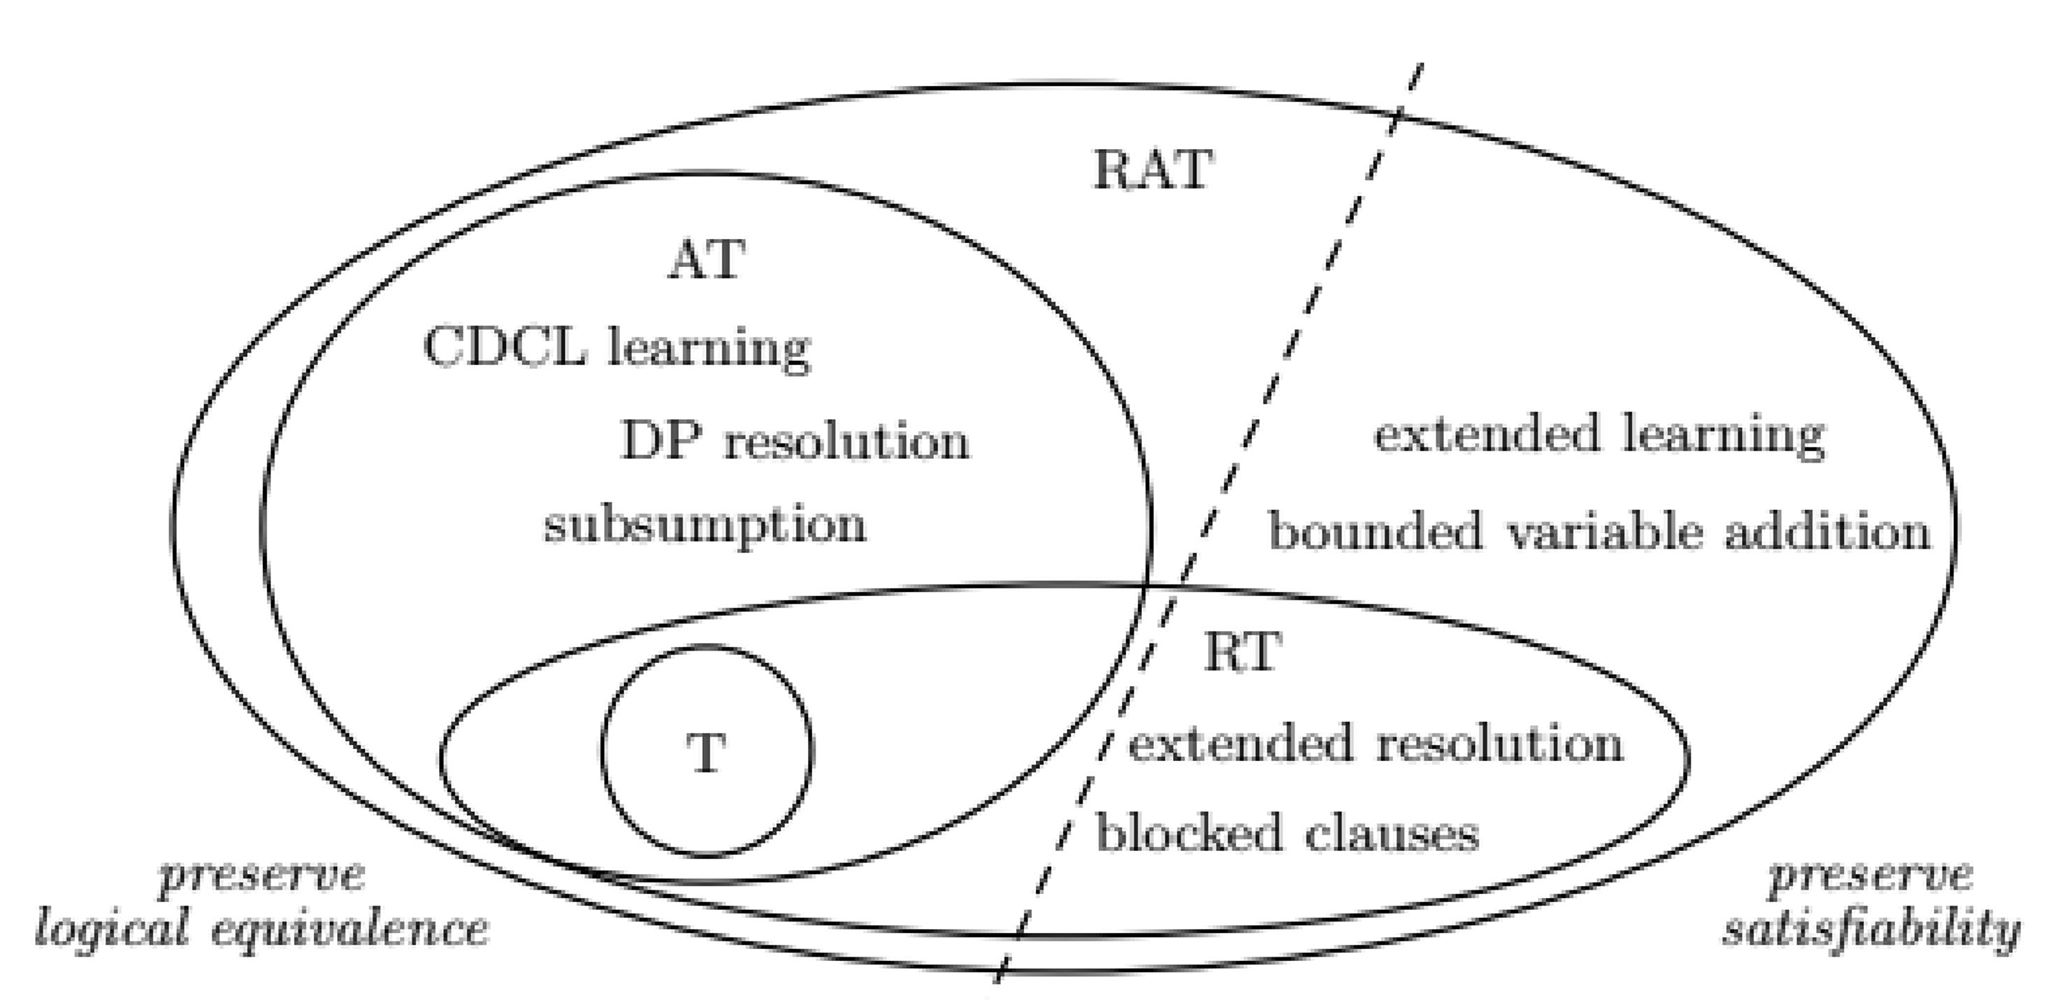
\includegraphics[width=\textwidth,height=0.8\textheight,keepaspectratio]{rat.jpg}
    \end{center}
\end{frame}

\begin{frame}
	\frametitle{Extended resolution}
    \begin{block}{Extension rule}
        Allows to iteratively add definitions of form $x := a \wedge b$ by adding caluses
        $(x \vee \neg a \vee \neg b) \wedge (\neg x \vee a) \wedge (\neg x \vee v)$.
    \end{block}


\end{frame}

\begin{frame}[t]
    \frametitle{Blocked clauses}

    \begin{block}{Blocked clause}
        Given formula $\varphi$, a clause $C$, and literal $l \in C$, the literal $l$
        blocks $C$ with respect to $\varphi$ if:
        \begin{enumerate}
            \item for each clause $D \in \varphi$ with $\neg l \in D$, $C \diamond_l D$
                  is tautology, or
            \item $\neg l \in C$, i.e., $C$ itself is tautology.
        \end{enumerate}
    \end{block}

    \pause
    \begin{block}{Example}
    $\varphi = (\neg b \vee c) \wedge (a \vee c) \wedge
                  (\neg a \vee b) \wedge (\neg a \vee \neg b) \wedge
                  (a \vee \neg b) \wedge (b \vee \neg c)
    $

    \bigskip
    $(\neg b \vee c)$ is blocked on $c$, because $(\neg b \vee c)
    \diamond_c (b \vee \neg c) = (\neg b \vee b)$.

    \bigskip
    Since $\varphi$ is unsatisfiable, $\varphi \setminus
    \{(\neg b \vee c)\}$ must be unsatisfiable.
    \end{block}

    \pause
    \textbf{Blocked clause addition} is generalization of extended resolution. May add clauses not logically implied by the formula.
\end{frame}

\begin{frame}
    \frametitle{Resolution Asymmetric Tautologies (RAT)}
    \begin{block}{Resolution asymmetric tautology}
    Clause $C$ has RAT on $l$  with respect to $\varphi$ if for all $D \in \varphi$ with $\neg l \in D$ holds that
    \[
        \varphi \wedge \neg C \wedge (\neg D \setminus (l)) \vdash_1 \emptyset
    \]
    \end{block}
    \pause
    RAT is generalization of RUP clauses:
    \[
        \varphi \wedge \neg C \vdash_1 \emptyset
        \implies \varphi \wedge \neg C \wedge (\neg D \setminus (l)) \vdash_1 \emptyset
    \]
    \pause
    and, if clause $C$ is blocked on $l$, then for all $D \in \varphi$ with $\neg l \in D$
    holds that $C$ contains a literal $k \neq l$ such that $\neg k \in D$, so:
    \[
        \varphi \wedge (k) \wedge (\neg k)  \vdash_1 \emptyset
        \implies \varphi \wedge \neg C \wedge (\neg D \setminus (l)) \vdash_1 \emptyset
    \]
\end{frame}

\begin{frame}
	\frametitle{Excursion to bounded variable addition}
	\begin{block}{Bounded variable addition}
		Adds new variable to express dependenties of variables in clauses and potentially shrinks the formula.
	\end{block}
	\begin{block}{Example}
        $
            \varphi = (\neg a \vee \neg b \vee \neg c) ~\wedge~ (a \vee d) ~\wedge~
  					  (a \vee e) ~\wedge~ (b \vee d) ~\wedge~ (b \vee e) ~\wedge~ (c \vee d)
		$

		\bigskip
		BVA introduces a new variable $f$.

		\bigskip
		$
			\varphi = (f \vee a) \wedge (f \vee b) \wedge (f \vee c) \wedge (\neg f \vee d)
					  \wedge (\neg f \vee e)
		$
	\end{block}

	\begin{itemize}
		\item Cannot be expressed  only with resolution steps.
	\end{itemize}
\end{frame}

\begin{frame}[t]
  \frametitle{Proofs with extended resolution -- RAT and DRAT}
    Extends RUP format with RAT lemmas.
	\begin{columns}[t]
	\begin{column}{0.6\textwidth}
        \begin{align*}
            \varphi =~& (\neg a \vee \neg b \vee \neg c) \wedge (a \vee d) ~\wedge~{} \\
  					  & (a \vee e) \wedge (b \vee d) \wedge (b \vee e) ~\wedge~{} \\
                      & (c \vee d) \wedge (c \vee e) \wedge (\neg d \vee \neg e)
        \end{align*}
		\begin{itemize}
			\item Uses BVA to replace first six clauses by five new cluses using a fresh new variable
			\item New clauses are RAT clauses.
			\item Final proof is only $\{(f),\emptyset\}$.
		\end{itemize}
	\end{column}
	\begin{column}{0.4\textwidth}
		\begin{table}[]
		\begin{tabular}{rrll}
		\textbf{} & 6  & 1 & 0 \\
		\textbf{} & 6  & 2 & 0 \\
		\textbf{} & 6  & 3 & 0 \\
		\textbf{} & -6 & 4 & 0 \\
		\textbf{} & -6 & 5 & 0 \\
		d         & 1  & 4 & 0 \\
		d         & 2  & 4 & 0 \\
		d         & 3  & 4 & 0 \\
		d         & 1  & 5 & 0 \\
		d         & 2  & 5 & 0 \\
		d         & 3  & 5 & 0 \\
				  &    & 6 & 0 \\
				  &    &   & 0
		\end{tabular}
		\end{table}
	\end{column}
	\end{columns}
\end{frame}

\begin{frame}[fragile]
  \frametitle{RAT checking}

    \begin{block}{Resolution asymmetric tautology}
    Clause $C$ has RAT on $l$  with respect to $\varphi$ if for all $D \in \varphi$ with $\neg l \in D$ holds that
    \[
        \varphi \wedge \neg C \wedge (\neg D \setminus (l)) \vdash_1 \emptyset
    \]
    \end{block}
\begin{lstlisting}
RATchecker(CNF formula $\varphi$, queue Q of lemmas)
  while Q is not empty
    L $\leftarrow$ Q.dequeue()
    if $\emptyset \not \in \text{BCP(}\varphi \wedge \neg \text{L}$) then <@\color{gray}{// check if L has AT}@>
      let $l$ be the first literal in L <@\color{gray}{// L has RAT on $l$}@>
      forall $\text{C} \in \varphi_{\neg l}$ do
        $\text{R} \leftarrow \text{C} \diamond \text{L}$
    	if $\emptyset \not \in \text{BCP(}\varphi \wedge \neg \text{R}$)
          return "checking failed"
    $\varphi \leftarrow \text{BCP(}\varphi \wedge \text{L}$)
    if $\emptyset \in \varphi$
      return UNSAT
  return "all lemmas validated"
\end{lstlisting}

%\pause
%\begin{itemize}
%	\item RAT checker is slower then RUP checker because of computing $\varphi_{\neg l}$.
%	\item But in practice $\varphi_{\neg l}$ is often empty.
%\end{itemize}
\end{frame}

\begin{frame}
	\frametitle{Some comparison}
    \begin{center}
        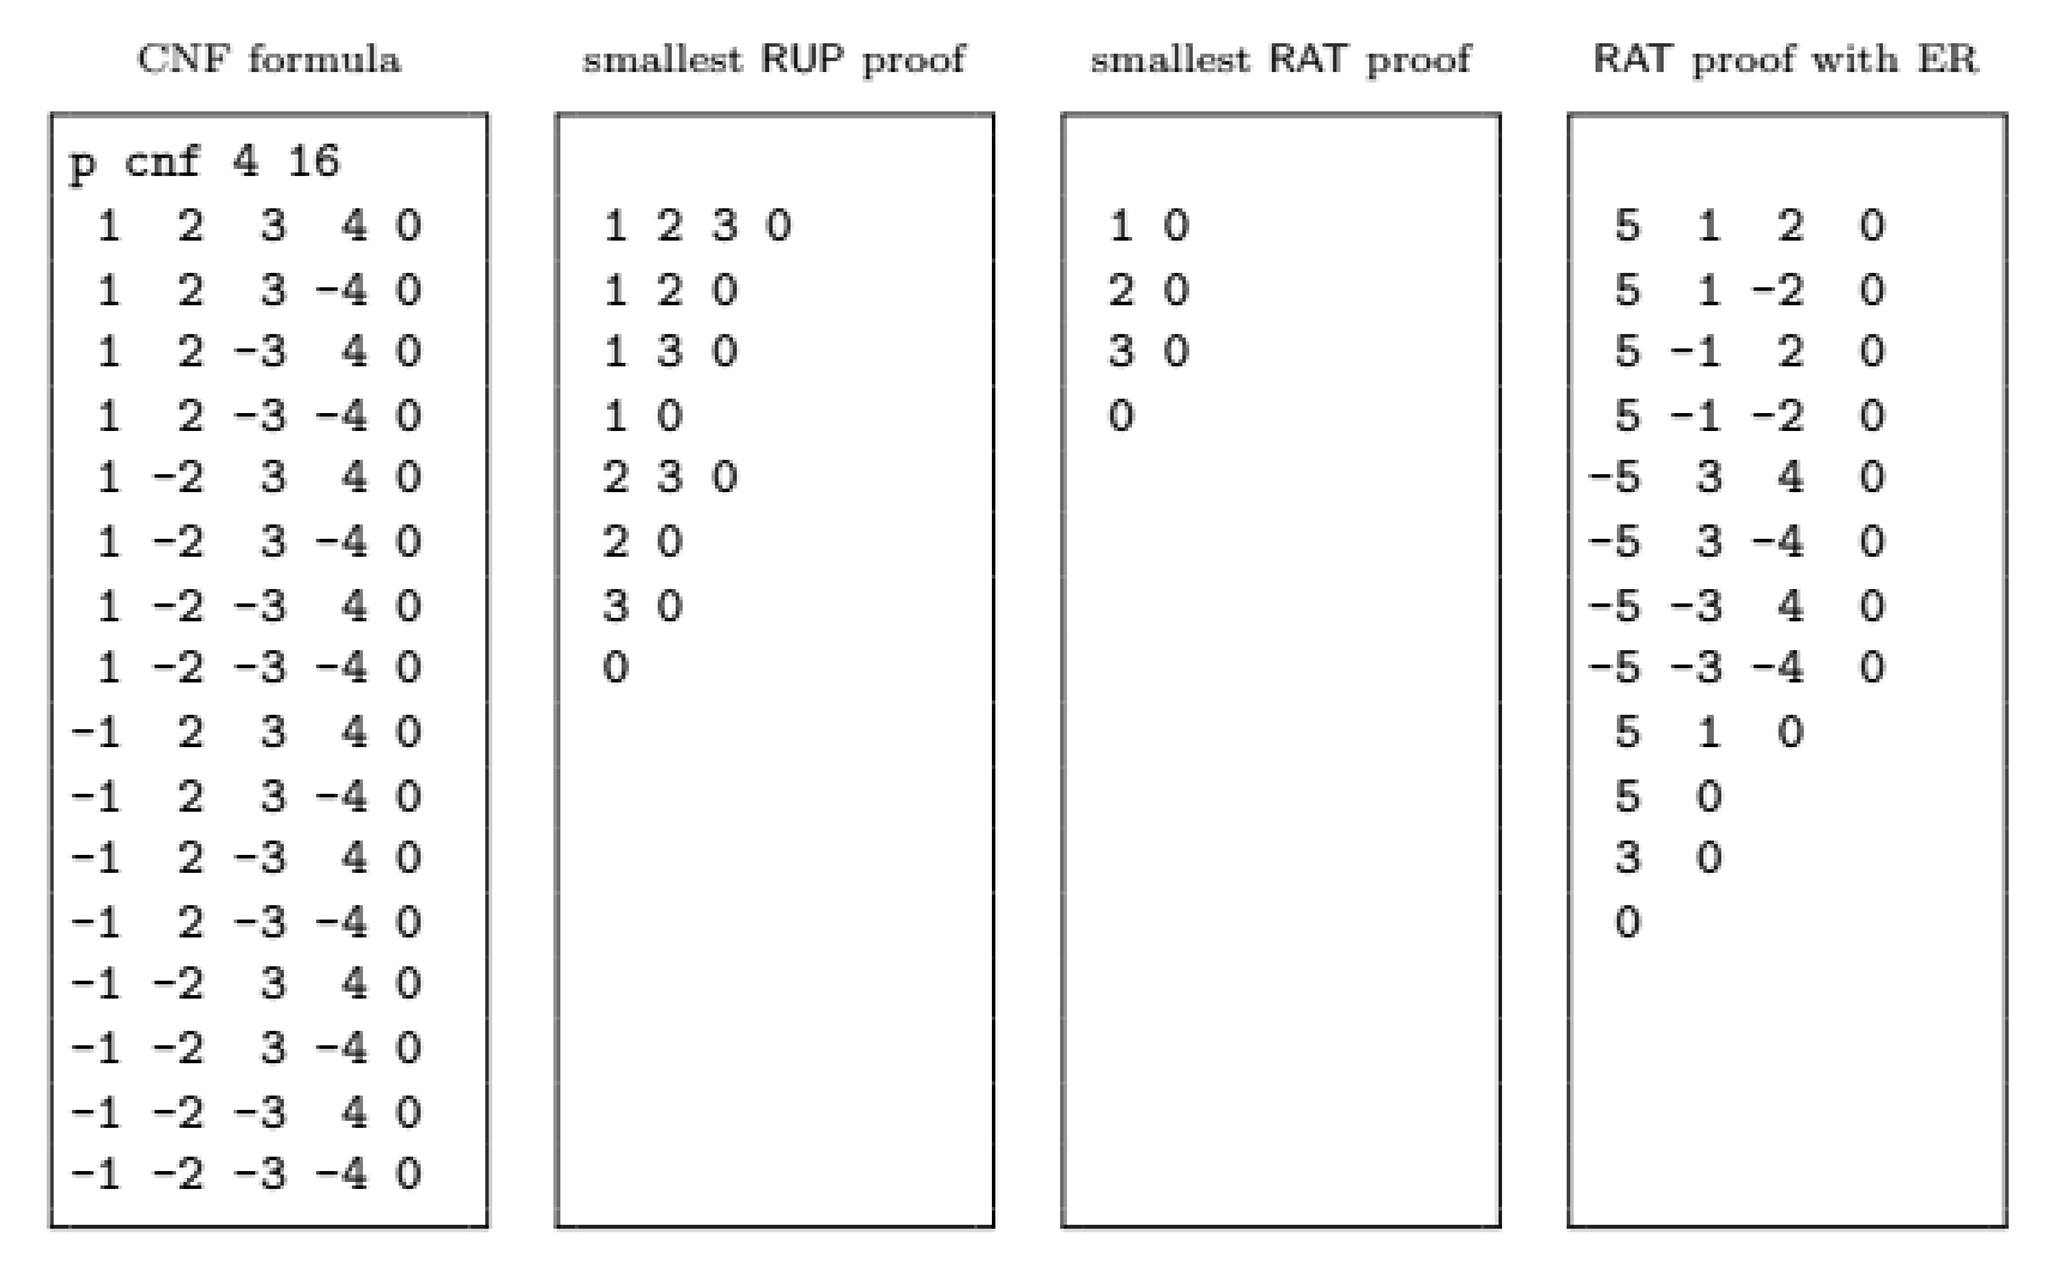
\includegraphics[width=\textwidth,height=0.8\textheight,keepaspectratio]{formats.jpg}
    \end{center}
\end{frame}

\begin{frame}
	\frametitle{Benchmarks}
    \begin{center}
        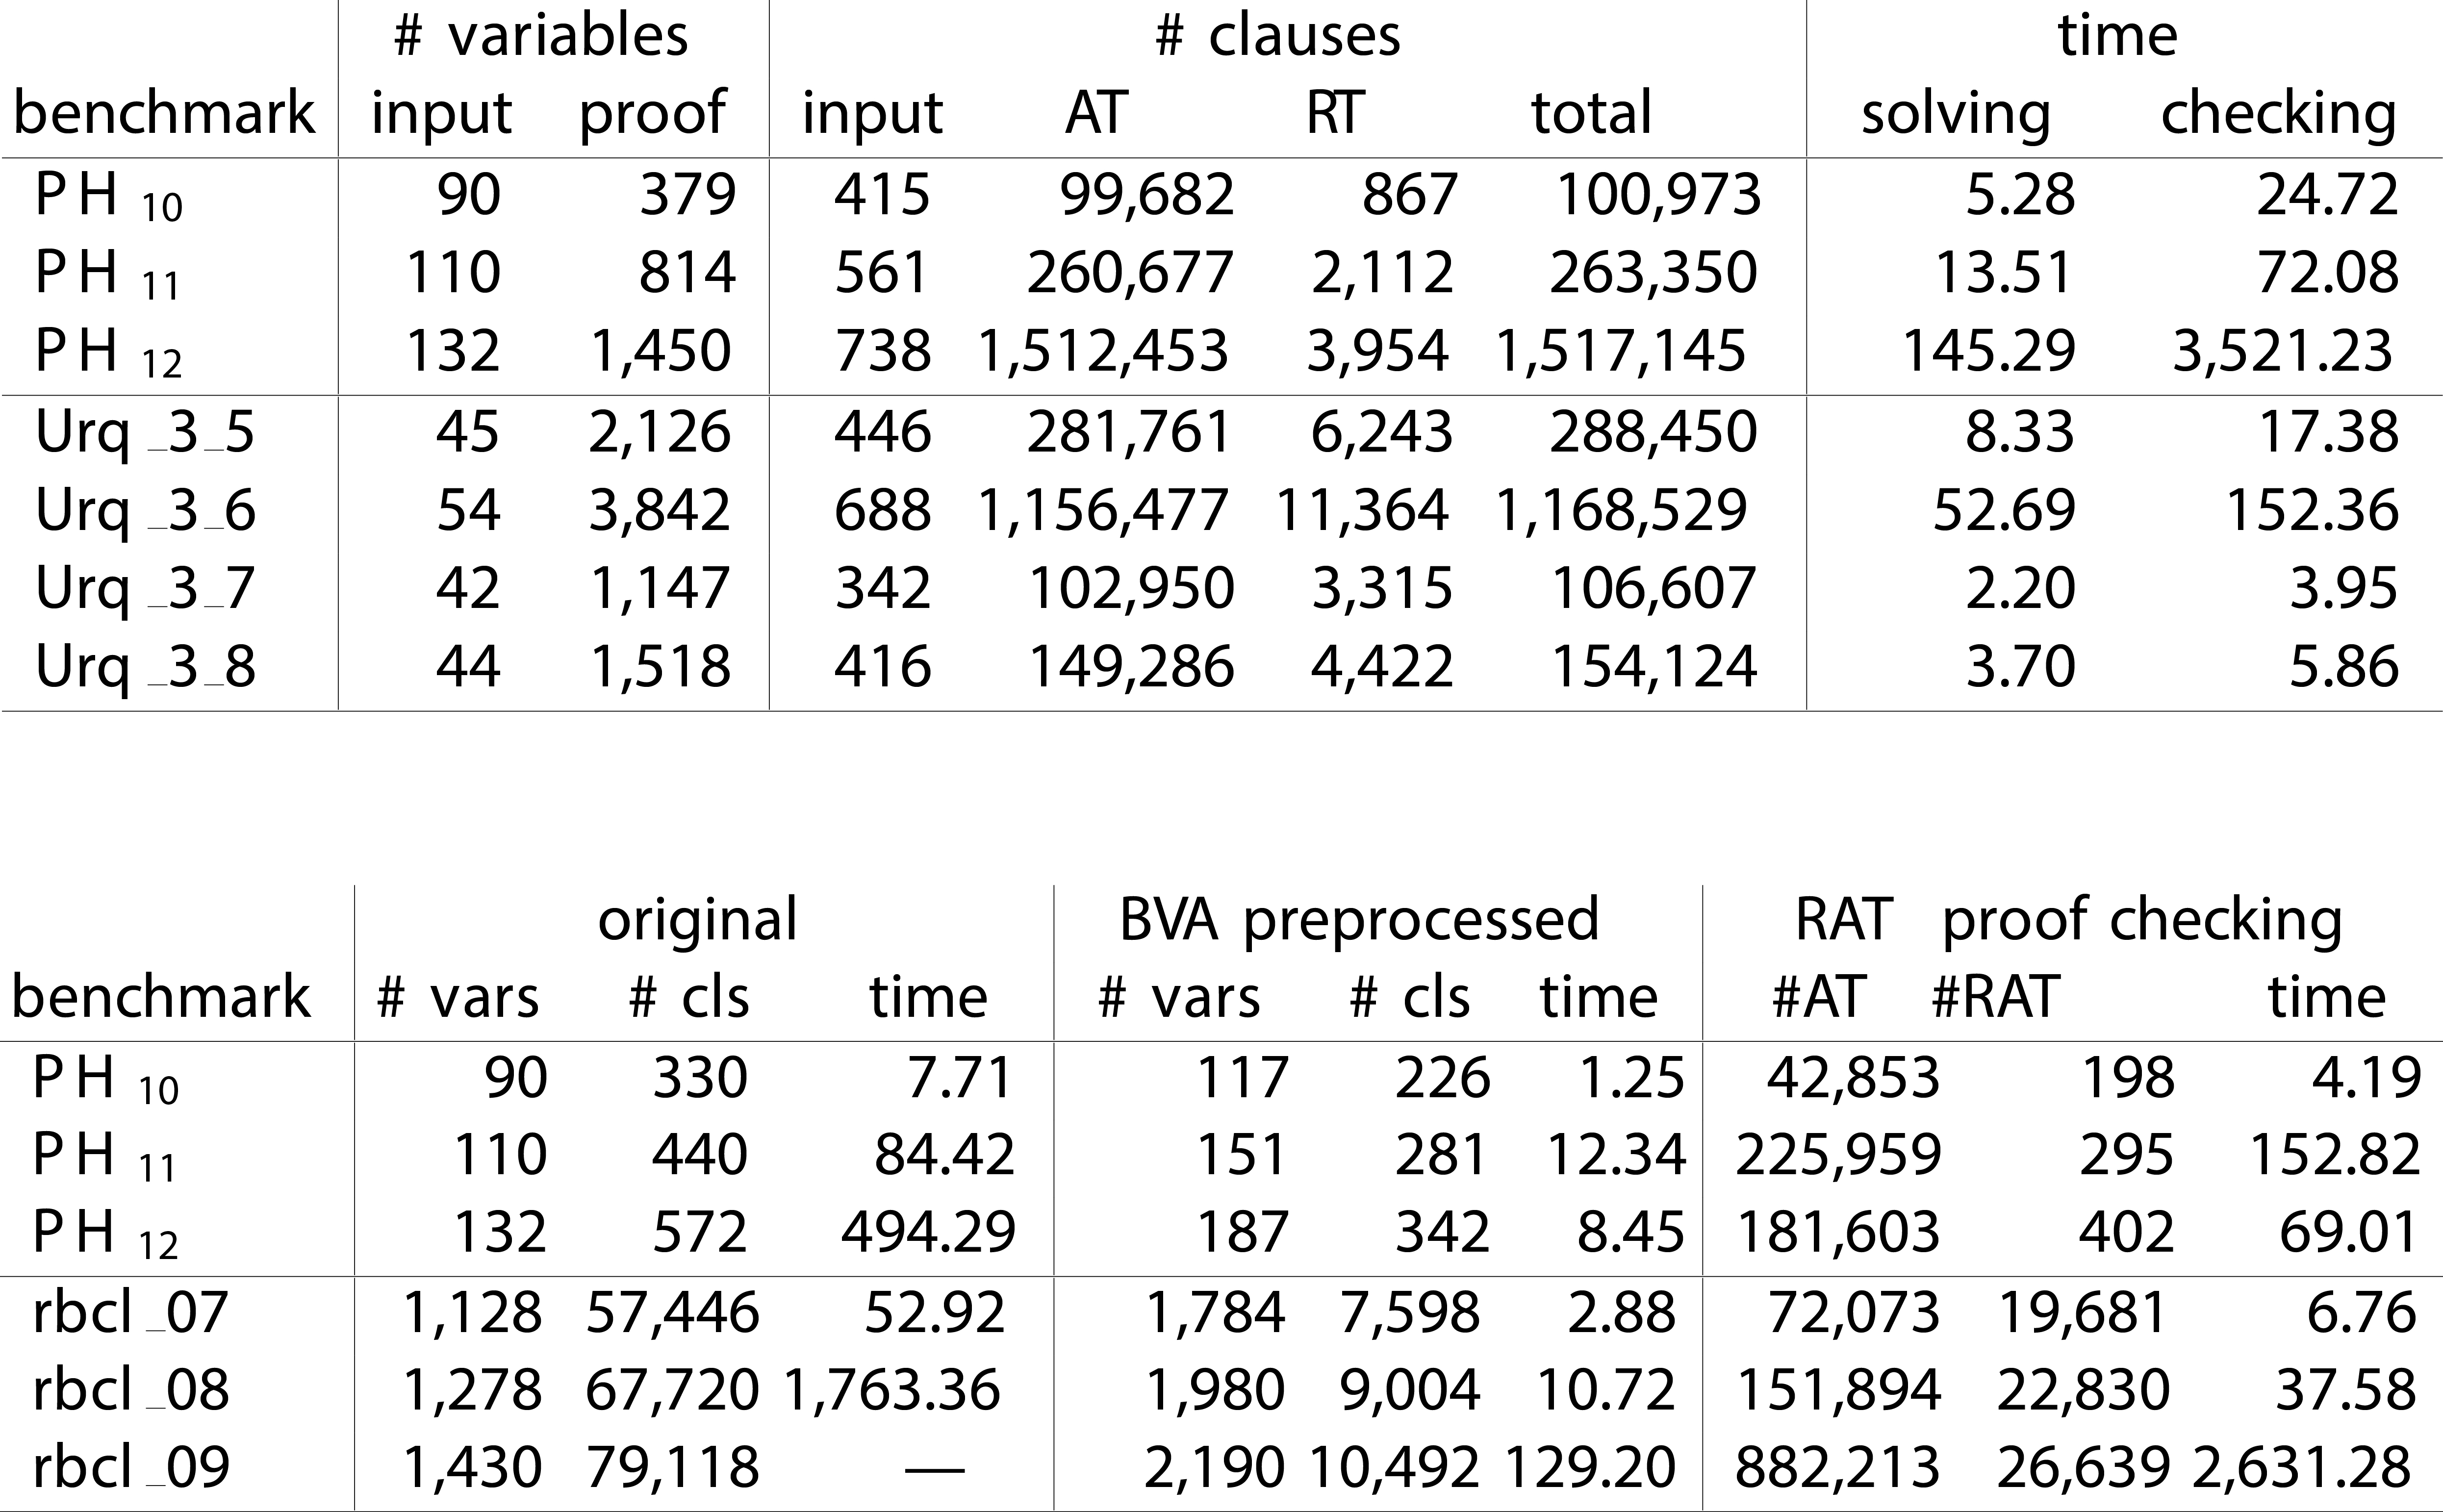
\includegraphics[width=\textwidth,height=0.8\textheight,keepaspectratio]{results.jpg}
    \end{center}
\end{frame}

\begin{frame}
	\frametitle{Proofs limitations}
	\begin{itemize}
		\item no method for easy extraction of unsatisfiability proofs from lookahead solvers
		\item how to handle preprocessing of formulas (Gaussian Elimination, Cardinality Resolution, Symmetry Breaking)
		\item no common API for proof manipulations
		\item extraction of resolution proof from clausal proof
		\item using clausal proofs for interpolants generation
	\end{itemize}
\end{frame}

\end{document}

%%% Local Variables:
%%% mode: latex
%%% TeX-master: t
%%% End:
